\documentclass[math]{cours}
\author{Clara Pinsard}
\title{Méthodologies Juridiques}
\date{2024-2025}
\begin{document}
\bettertitle
\section*{Introduction}
Au cours des 12 séances, on se concentre sur 3 exercices principaux:
\begin{enumerate}
	\item La dissertation Juridique
	\item Le commentaire d'arrêts, de décisions, de textes (constitutions,).
	      On s'attardera longuement dessus.
	\item Le cas pratique: l'objectif est ici d'apporter une solution juridique à une situation composée de fait.
\end{enumerate}

La validation prend en compte:
\begin{itemize}
	\item La participation au long du semestre,
	\item Un exercice intermédiaire facultatif à rendre à l'une des séances,
	\item Un exercice final obligatoire au choix parmi les trois à rendre à la dernière séance.
\end{itemize}

\section*{Les outils du juriste}
\subsection*{Ressources Primaires}
En ligne:
\begin{itemize}
	\item Légifrance regroupe les lois, décrets et jurisprudences.
	\item Les sites des juridictions internes: cour de cassation, conseil d'état, conseil constitutionnel
	\item \url{eur-lex.europa.eu} pour le droit de l'Union Européenne
\end{itemize}

Les codes édités par Lexi Nexis et Dalloz par exemple.
Un article du code civil se présente avec les informations suivantes:
\begin{itemize}
	\item Son numéro
	\item La loi qui l'a créé
	\item Ses alinéas
	\item Ses références textuelles, i.e. les articles proches dans d'autre codes
	\item Ses références doctrinales. La doctrine est l'ensemble des personnes qui font des recherches en droit.
	      Les références doctrinales permettent donc de compléter le commentaire de l'article.
	\item Sous l'article se trouvent des jurisprudences qui viennent préciser le droit consacré.
\end{itemize}


\subsection*{Les Ressources Secondaires}
Comme ressources secondaires on trouve:
\begin{itemize}
	\item Les recueils de jurisprudence: GAJA, GAJC (grands arrêts de la justice administrative et civile)
	\item Les revues:
	      \begin{itemize}
		      \item Hebdomadaires: Lextenso, Lexisnexis (la semaine juridique: actualités juridiques: générale: JCPG, entreprise: JCPE, notariat: JCPN), Dalloz (recueil Dalloz: D.), Lamy (RCDC)
		      \item Trimestrielles: revue trimestrielle de droit civil et commerciale
		      \item Semestrielles: Titre VII (revue numérique du Conseil Constitutionnel).
	      \end{itemize}
	\item Les manuels et encyclopédies
\end{itemize}

\section{Introduction au Raisonnement Juridique}
\subsection{Le Syllogisme Juridique}
On utilise une forme de base de la logique aristotélicienne: on a deux propositions, une majeure et une mineure qu'on rapproche pour tirer une conclusion.
Ici, on n'a pas vraiment des propositions mais des prescriptions.
Le syllogisme est composé de trois étapes:
\begin{enumerate}
	\item La majeure: L'affirmation d'une norme applicable,
	\item La mineure: La confrontation de la norme aux faits,
	\item La conclusion: quant à l'applicabilité de la norme.
\end{enumerate}

% TODO: insérer exemple consentement contrat
Par exemple, pour un contrat conclus sans consentement d'une des parties:


\subsection{Les difficultés de mise en oeuvre du syllogisme juridique}
Il est nécessaire pour appliquer le syllogisme de connaître la règle applicable, mais aussi des conditions de son application.
\begin{quote}
	La théorie générale du droit se distingue aussi de la méthodologie juridique qui envisage les moyens de résolution des problèmes pratiques rencontrés par les juristes, tels que les méthodes d'interprétation des énoncés normatifs ou les critères d'identification et de résolution des antinomies: des conflits entre règles de droits.
	\begin{flushright}
		Eric \textsc{Millard}, Théorie Générale du Droit aux éditions Dalloz
	\end{flushright}

\end{quote}

Il y a donc trois grands problèmes juridiques:
\begin{enumerate}
	\item L'obscurité de la règle: liée notamment aux termes techniques peu connus utilisés parfois en droit, et en même temps à l'utilisation de termes courants parfois mal définis.
	      À propos, on pourraît poser la question de l'interprétation du mot \textit{vehicle} sur un panneau \textit{No vehicle in the park}, suivant Herbert Hart.
	\item Le nombre de règles applicables: on utilise une hiérarchie des normes pour limiter les conflits entre des sources de droit différentes.
	\item Le cas où aucune règle ne s'applique: Auquel cas on doit interpréter une autre règle pour trouver une solution.
	      Ceci découle parfois de la distinction de vitesses d'évolution entre le droit et la société.
\end{enumerate}
Il y a donc notamment des problèmes liés à l'identification de la règle applicable.

\subsection{L'identification de la règle applicable par l'interprétation}
Les juristes ont proposés différentes solutions pour interpréter le droit.
Ces solutions ont deux grands objectifs communs:
\begin{enumerate}
	\item Garantir la compatibilité des normes: éviter des contradictions apparentes
	\item Garantir la complétude des normes: éviter les vides juridiques
\end{enumerate}
Pour arriver à leurs fins, les juristes proposent des méthodes générales:
\begin{enumerate}
	\item Des techniques d'interprétations: des procédés et maximes interprétatitves
	\item Des modèles d'interprétation
\end{enumerate}

On peut trouver trois principaux procédés d'interprétation:
\begin{description}
	\item[L'interprétation \textit{a pari}]
	      Celle-ci se fait par analogie, ou à une situation, ou aux effets d'une autre décision.
	      Par exemple: pour l'application des règles du divorce à l'annulation du mariage.
	      L'analogie intervient alors au niveau des effets.
	      Cette interprétation ne peut pas avoir lieu en droit pénal, et ce, parce que le droit pénal est fondé sur le fait qu'il n'y a pas d'infraction sans texte.

	\item[L'interprétation \textit{a fortiori}]
	      Celle-ci est possible lorsque la raison d'être de la règle se retrouve avec plus de force encore dans le cas non prévu par le texte.
	      Par exemple, si un hôtel interdit de séjourner dans son établissement avec un animal domestique, \textit{à fortiori}, il est interdit d'y séjourner en compagnie d'un animal sauvage.

	\item[L'interprétation \textit{a contrario}]
	      Si un objet est inclu dans une règle de droit, en particulier, on considère que le contraire en est exclu.
	      Par exemple, l'article 6 du code civil dit:
	      \begin{quote}
		      On ne peut déroger par des conventions particulières aux lois qui intéressent l'ordre public et les bonnes m\oe urs.
	      \end{quote}
	      On en déduit \textit{à contrario} un principe de liberté contractuelle: il est possible de déroger aux lois qui ne sont dictées ni par l'ordre public ni par les bonnes m\oe urs.
	      De même: le droit pénal réprime certains comportements, à contrario, il est impossible de réprimer un comportement non prévu par le droit pénal.
\end{description}
Il y a parfois plusieurs possibilités d'interprétation.
Celle que l'on retiendra est la plus cohérente vis-à-vis de l'environnement.
Le juge tranche, possiblement en cherchant l'intention de l'auteur de la règle.

Les maximes d'interprétation sont des principes généraux qui ne sont pas écrits, mais qui sont souvent appliqués en droit français.
Elles sont retrouvées dans plusieurs domaines du droit.
Par exemple:
\begin{itemize}
	\item \textit{Les lois spéciales dérogent aux lois générales}: des régimes plus précis s'appliquent à la place de régimes plus généraux.
	      Par exemple, les droits spéciaux des contrats (vente, pacs) dérogent au droit commun des contrats.
	\item \textit{Les exceptions doivent être strictement interprétées}:
	      Par exemple, le principe en droit des contrats est la capacité de contracter.
	      La liste des exceptions prévues à l'article 1146 du Code civil (mineurs non émancipés et majeurs protégés) ne doit pas être allongée.
	\item Il y a d'autres maximes inutiles mais souvent mentionnées par les juristes: \textit{Ce qui est clair ne s'interprète pas}.
\end{itemize}

Pour les cas plus généraux, on a des modèles d'interprétation:
\begin{description}
	\item[L'Exégèse] C'est un modèle français de droit civil, fondé sur l'interprétation de Portalis.
	      Le modèle considère que le droit est un texte sacré.
	      Il part du principe qu'il suffit de lire le droit pour connaître le droit, le code civil se suffisant à lui même, en se fondant sur l'interprétation littérale.
	      Il a une forte importance sur l'enseignement du droit, centré sur le code civil.
	      Il arrive que certains professeurs ne fassent que lire le code civil en le commentant légèrement.
	      Dans ce modèle, la loi est complète, tout est dans la loi, et toute difficulté peut être résolue en se référant au code civil.
	      Ce modèle s'affirme notamment politiquement neutre.
	      L'affirmation de neutralité est une affirmation de légitimation.
	      Les personnes qui soutiennent l'exégèse sont conservateurs, et l'idée de ne pas se référer à d'autres éléments est à l'origine du conservatisme juridique.
	      L'idée est que ce qui est du droit a déjà été prévu.
	      À partir de la fin du 19ème siècle on a commencé à se questionner sur une possible ouverture théorique.
	\item[La Libre Recherche Scientifique] C'est un modèle réactionnaire à l'exégèse, qui apparaît fin 19ème.
	      Il se fonde sur l'idée que pour interpréter le droit, il faut le replacer dans le monde social et scientifique.
	      Il a été porté notamment par François Geny (Doyen de la faculté de droit de Nancy, protagoniste du mouvement des \emph{Juristes Inquiets}, dont le but était de réformer le code civil tout en adhérant aux idées qu'il porte.
	      Pour l'auteur, le texte ne peut être sollicité à l'infini, et il faut s'intéresser au contexte)
	      et par Maurice Hauriou (grand arrêtiste travaillant sur le droit administratif, partie du droit publique construite sans code, contrairement au droit civil.
	      Il rejette complètement l'exégèse et souhaite intégrer la sociologie au droit. Pour lui, la sociologie peut être utilisée pour interpréter le droit.).
	      Pour cette école de pensée, le juge doit évaluer le droit en prenant en compte des données sociales, historiques.
	      Le rôle du juge est bien plus important dans ce modèle.
	      La puissance est donné au juge plus qu'au législateur.
	\item[L'interprétation Téléogique] C'est un modèle qui considère l'interprétation du droit en fonction de l'objectif de la règle.
	\item[L'interprétation Évolutive] C'est un modèle qui considère que le droit évolue en s'adaptant au contexte contemporain.
\end{description}

En Suisse, l'article premier dit que le juge a le pouvoir de faire acte de législateur, c'est une approbation claire de la méthode de la Libre Recherche Scientifique.
Ce n'est pas du tout ce que prévoit le code civil en France, où le juge n'a pas le droit d'agir comme législateur.

\begin{quote}
	\begin{center}
		Article 4 du Code Civil
	\end{center}
	{\it	Le juge qui refusera de juger, sous prétexte du silence, de l'obscurité ou de l'insuffisance de la loi, pourra être poursuivi comme coupable de déni de justice.}
	\begin{center}
		Article 5 du Code Civil
	\end{center}
	{\it	Il est défendu aux juges de prononcer par voie de disposition générale et réglementaire sur les causes qui leur sont soumises.}
\end{quote}

Ces deux articles sont les seuls permettant de mieux cadrer les pouvoirs des juges.
Le second prohibe les arrêts de réglements, arrêts suffisamment généraux et abstraits pour s'appliquer exactement dans d'autres cas.
Le juge ne doit pas faire d'interprétation générale de la loi, et ne peut juger que sur la situation qui lui est présentée.
Toutefois, les juges des hautes cours proposent très souvent des décisions assez générales pour qu'elles puissent s'appliquer plus tard (et parfois le disent même).
Il faut relativiser l'article 5, notamment dans des matières qui n'ont été que peu réformées, par exemple en responsabilité civile: il y a 6 articles dans le code civil au total.
Sur les 15 dernières années, on se retrouve face à une inflation législative et décrétale très importante, car le droit agit énormément plus sur des sujets techniques.
Le juge ne s'exprime pas, n'interprète pas de la même manière selon le domaine.
Plus la loi est précise, plus le juge est lié.

\subsection{Les différences de raisonnement selon les différentes professions juridiques}
Pour les différentes professions du milieu juridique, une fois que le problème de l'interprétation juridique est résolu, comment appliquer le syllogisme juridique ?
L'existence de multiples interprétations du droit sert l'application du droit.
Il s'agit toujours de questions d'argumentation.
Il y a donc différentes manières d'appliquer le syllogisme selon la profession de l'écosystème juridique:
\begin{description}
	\item[L'avocat] Il part de la solution qui est dans l'intérêt de son client (conclusion) pour trouver une règle applicable aux faits (majeure du syllogisme)
	\item[Le juge] En principe, il juge en suivant le syllogisme, et donc en partant d'une règle de droit pour l'appliquer aux faits.
	      Dans l'article 12 du code de procédure civile, il est écrit que \textit{Le juge tranche le litige conformément aux règles de droit qui lui sont applicables}.
	      Il faut qu'il y ait une permanence des décisions, pour que les droits qui sont garantis le restent dans le temps.
	      Il est en réalité complètement illusoire de penser que le juge ne compte que sur la règle de droit.
	      Il y a déjà des questions d'interprétation, mais également le fait que le juge, est un humain et a sa propre conception du juge.
	      L'article 12 proscrit le jugement en équité (selon la conception qu'à le juge du juste), mais il arrive des exceptions, notamment en droit privé, où des articles (par exemple l'article 700 du code de procédure civile) prévoient cette possibilité pour le juge.
	      \begin{quote}
		      \begin{center}
			      Article 700 du Code de Procédure Civile
		      \end{center}
		      {\it Le juge condamne la partie tenue aux dépens ou qui perd son procès à payer:
		      \begin{enumerate}
			      \item A l'autre partie la somme qu'il détermine, au titre des frais exposés et non compris dans les dépens;
			      \item Et, le cas échéant, à l'avocat du bénéficiaire de l'aide juridictionnelle
			            partielle ou totale une somme au titre des honoraires et frais,
			            non compris dans les dépens,
			            que le bénéficiaire de l'aide aurait exposés s'il n'avait pas eu cette aide.
			            Dans ce cas, il est procédé comme il est dit aux alinéas 3 et 4 de l'article 37 de la loi n°01-647 du 10 juillet 1991.
		      \end{enumerate}
		      Dans tous les cas, le juge tient compte de l'équité ou de la situation économique de la partie condamnée.
		      Il peut, même d'office, pour des raison tirées des mêmes considérations, dire qu'il n'y a pas lieu à ces condamnations.
		      Néanmoins, s'il alloue une somme au titre du 2° du présent article, celle-ci ne peut être inférieure à la part contributive de l'État.
		      }
	      \end{quote}
	      Le principe de base est que la partie qui perd sont procès à payer les frais de celui-ci (les dépens, définis à l'article 695 de ce même code ainsi que d'autres frais).
	      Dans les frais exposés et non compris pour les dépens, on a par exemple le manque à gagner lié au fait pour une partie de participer personnellement aux opérations de procédure, en l'espèce une perte de salaire.
	      Il y a (rarement) eu également la prise en compte du préjudice moral occasionné par les \textit{peines et tracas du procès}.
	      Il peut y avoir des dérives: si le montant est trop élevé, il y a punition de la partie perdante et atteinte au droit à exercer la justice.
	      Si au contraire le montant est trop faible, il ne couvrirait pas les frais de procédure de la partie gagnante.
	      Une solution serait d'objectiver les frais de procédure, ce qui est difficile de part la nécessité de solvabilité de la partie perdante.
\end{description}


\section{La justice judiciaire}
\subsection{Introduction}
La justice française est extrêmement critiquée: sondage Ifop Express traduit un manque de confiance (47\% seulement considèrent les juges impartiaux, 53\% seulement font confiance à la justice et 62\% considèrent que la justice fonctionne mal).
Au vu de ces constats, de nombreuses réformes se sont mises en place:
\begin{itemize}
	\item Loi J21 de 2016 de modernisation de la justice du XXIème siècle qui réforme en profondeur des contentieux pour désengorger les tribunaux.
	      Les 60000 dossiers de contentieux de divorces par an peuvent maintenant se faire par consentement mutuel sans juge.
	      On a créé une procédure sans juge qui crée des risques de contentieux post-divorce.
	\item Les chantiers de la justice (Belloubet et Philippe) en 2017:
	      projet assez général de transformation numérique, de simplification des procédures civiles et pénales, l'adaptation de l'organisation territoriale ainsi que la refonte du sens et de l'efficacité des peines
	\item Réforme en 2023 d'orientation et de programmation du ministère de la justice 2023-2027:
	      hausse du budget de la justice, autorisation de réforme de la procédure pénale par ordonnance, expérimentation des tribunaux des activités économiques
\end{itemize}

\subsection{L'ordre judiciaire}
Il y a trois niveaux:
\begin{enumerate}
	\item Les Tribunaux de première instance jugent en fait et en droit
	\item Les Cours d'appel jugent en fait et en droit
	\item La Cour de cassation juge en droit
\end{enumerate}

Il y a deux principes fondamentaux concernant l'organisation de l'ordre judiciaire:
\begin{description}
	\item[Le double degré de juridiction:]
	      un demandeur qui a perdu son procès en première instance peut demander, sauf exception (demandes concernant des sommes de moins de 5000€),
	      à faire juger de nouveau son affaire.
	      \begin{quote}
		      L'appel est une garantie de bonne administration de la justice.
		      \begin{flushright}
			      Muriel \textsc{Fabre-Magnan}, \textit{Introduction générale au droit}
		      \end{flushright}
	      \end{quote}
	      Il est donc notamment interdit de faire de nouvelles demandes en appel.
	      On ne peut pas faire valoir de moyens nouveaux en appel.
	\item[La distinction juges du fond/juges du droit:]
	      le fait relève du \emph{pouvoir souverain des juges} ou de l'\emph{appréciation souveraine des juges du fond}.
	      Juger le fait, c'est apprécier la valeur probante du fait:
	      \begin{quote}
		      [En droit, il faut] retenir la preuve \emph{la plus solide ou moins vulnérable}
		      \begin{flushright}
			      Henri \textsc{Batiffol}, \textit{Observations sur la preuve des faits}
		      \end{flushright}

	      \end{quote}
	      \begin{quote}
		      On appelle preuve ce qui persuade l'esprit d'une vérité.
		      \begin{flushright}
			      Jean \textsc{Domat}
		      \end{flushright}

	      \end{quote}
	      Il n'y a donc pas de problème, sur le principe de jugement des faits, à distinguer le droit et le fon.
	      La qualification juridique c'est donner aux faits la règle de droit à appliquer, les catégoriser.
	      C'est une opération entre le fond et le droit.
	      Le contrôle effectué par la Cour de cassation va donc varier en fonction de la teinte factuelle de la qualification.
	      Celle-ci va donc parfois s'abstenir de contrôler la qualification pour des questions de politique juridique.
	      Par exemple, dans une décision de la chambre sociale du 20 décembre 2001 sur la qualification ou non du suicide d'un employé sur son lieu de travail comme accident de travail,
	      celle-ci a considéré que la qualification dépendait de l'\emph{appréciation souveraine des juges du fond}.
	      Selon le professeur Pierre-Yves Verkindt, cette décision était attendu de part l'affaiblissement du contrôle de la Cour de cassation depuis quelques années.
	      Ceci pose donc la question de la limitation des pouvoirs et du contrôle de la cour de cassation.
\end{description}

\subsection{L'ordre Judiciaire}

\begin{figure}[h]
	\centering
	L'ordre judiciaire est la partie gauche de l'organigramme ci-dessous.
	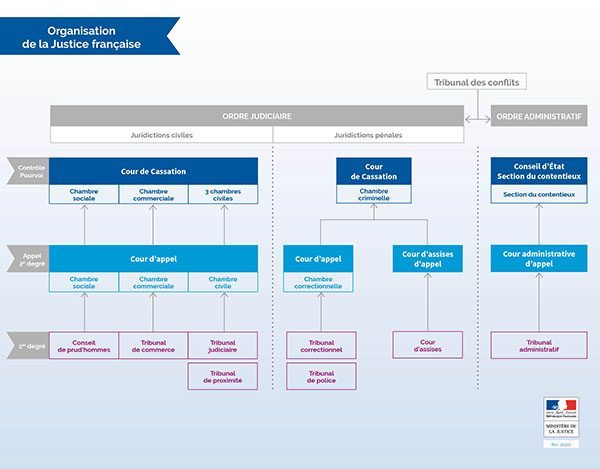
\includegraphics{orga_juridictionnelle}
	\caption{Composition de l'Ordre Judiciaire}
	\label{fig:ordre_judiciaire}
\end{figure}
\begin{definition}
	Les magistrats du siège rendent les décisions de justice.
	Ils sont inamovibles, indépendants, impartiaux.
	\label{def:siege}
\end{definition}
\begin{definition}
	Les magistrats du parquet, regroupé sous le ministère public.
	Ils requièrent la bonne application de la loi afin de protéger les intérêts de la société selon une politique gouvernementale.
	Ils sont indépendants, indivisibles, soumis à la politique du ministère de la justice.
	\label{def:parquet}
\end{definition}

\begin{remarque}
	Un magistrat du parquet décide de faire entrer des faits ou non dans la juridiction:
	Il va classer les infractions.
	Il peut décider de ne pas agir, de faire un rappel à la loi, ou de lancer une enquête.
	Ils ont donc une marge de manoeuvre, mais suivent globalement la politique gouvernementale.
\end{remarque}

\subsubsection{Les Juridictions du Premier Degré}
\paragraph{Les Juridictions Civiles}
\begin{description}
	\item[Tribunal Judiciaire] Création par la loi n°2019-222 du 23 Mars 2019 de programmation 2018-2022
	      Compétences:
	      \begin{itemize}
		      \item d'attribution:
		            tous les litiges dont la loi n'a pas confié la connaissance à une autre juridiction
		      \item territoriale:
		            tribunal du défender
	      \end{itemize}
	      Avant, il y avait les tribunaux d'instance et les tribunaux de grande instance qui se partageaient les compétences du TJ selon la valeur (si estimable a priori) du litige.
	      Il est composé d'un président, d'un procureur de la république et d'un magistrat du siège et du parquet.
	\item[Tribunal de commerce] Compétent pour les litiges entre commerçants ou relatif aux actes de commerce.
	\item[Conseil de prud'hommes] Compétent pour les litiges entre salariés et employeurs relatifs au contrat de travail
	\item[Tribunal paritaire des baux ruraux] Litiges entre propriétaires et exploitants de terres relatifs à un bail rural
	\item[Tribunal des Activités Économiques] À partir de 2025, les trois tribunaux ci-dessus vont être regroupés dans une expérience.
	\item[Tribunal des Affaires Sociales] Compétent pour les affaires concernant la sécurité sociale.
\end{description}

\paragraph{Les Juridictions Pénales}
Leurs distinctions sont fondées entre la distinction légale entre Crimes, Délits et Contraventions.
Il s'agit d'une échelle de gravité.
Le principe qui régit le droit pénal est l'article 8 de la DDHC: le principe de légalité des délits et des peines: \textit{Nullum crimen, nulla poena, sine lege}.
La justice pénale fonctionne en trois étapes:
\begin{enumerate}
	\item Poursuite: Le ministère public décide de l'opportunité des poursuites.
	\item Instruction: Elle est obligatoire en matière criminelle, facultative en correctionnelle et exceptionnelle en matière contraventionnelle.
	\item Jugement
\end{enumerate}

Une fois le stade du jugement atteint:
\begin{description}
	\item[Tribunaux Ordinaires] \begin{description}
		      \item[Tribunal de Police] Juge les contraventions de toutes classes et les infractions passibles de moins de 3000 euros d'amende
		      \item[Tribunal Correctionnel] Juge les délits et certaines infractions autres (par exemple financières)
		      \item[Cour d'assises] Juge les Crimes
	      \end{description}
	\item[Tribunaux Spéciaux] Il y en a dépendamment de la qualité du prévenu et de la potentielle partie civile:
	      \begin{description}
		      \item[Pour les Mineurs]
	      \end{description}
\end{description}

\subsubsection{Les Juridictions du Second Degré}
Ces juridictions sont les Cours d'appel, et sont, en France, un véritable degré de jugement.
La procédure d'appel est prévue par les articles 563 et suivants du code de Procédure Civile, qui permettent de produire de nouvelles pièces, de nouvelles preuves mais pas de nouvelles demandes.
Elles peuvent réformer le jugement comme l'annuler quand il y a atteinte aux conditions de validité du jugement (par exemple en cas de non respect du principe du contradictoire).
L'appel est:
\begin{itemize}
	\item Suspensif:
	      le délai d'un mois pour faire appel suspend l'exécution du jugement, sauf quand le jugement prescrit des mesures provisoires ou conservatoires
	\item Dévolutif:
	      la cour d'appel rejuge le litige dans son intégralité, donc en droit \textbf{et} en fait, mais seulement sur les points critiqués par l'appelant.
\end{itemize}
On appelle \emph{appelant} celui qui entame la procédure, \emph{intimé} celui qui est engagé dans la procédure, et on appelle \emph{conseiller} le magistrat.

\subsubsection{La Cour de cassation}
Elle siège au 5 quai de l'Horloge à Paris, il s'y déroule des conférences.
Sur la composition de la Cour:
\begin{itemize}
	\item Elle est présidée par un premier président, appelé premier magistrat judiciaire de France ou \emph{Premier}.
	\item Elle est composée de conseiller nommés par le conseil supérieur de la magistrature.
	      Avant, ils étaient nommés par le PR, puis par le CSM présidé par le PR, et enfin, le PR a été exclu de cet organe.
	      Chacune des formations du CSM est présidé par le Premier et par le Procureur Général.
	\item Elle est divisée en 6 chambres qui interviennent sur des affaires différantes (la premiere chambre civile (droit des personnes, de la famille, de la propriété intellectuelle, de la protection des consommateurs), la deuxième chambre civile (procédure civile, sécurité sociale, surendettement des particuliers), la troisième chambre civile (matière immobilière, environnement et pollution) une chambre sociale, une chambre commerciale financière et économique et une chambre criminelle)
	\item Elle comporte une chambre mixte pour les cas plus complexes.
	\item Lorsque la première cour d'appel de renvoi a refusé de s'incliner devant la solution de la Cour de cassation, l'assemblée plénière est saisie.
	      Elle peut aussi être saisie sur requête du Premier ou du PG, s'il y a un risque d'incohérence entre les arrêts de fond et de la Cour de cassation.
	\item Enfin, il y a une formation qui est chargée de répondre aux saisines sur avis.
	      Il y a une forme d'autorité de la Cour de cassation sur l'interprétation de la jurisprudence.
\end{itemize}
Le pourvoi en cassation n'est pas suspensif.
La Cour de cassation a pour rôle (au sein de l'ordre judiciaire) de juger les décisions de justice rendues en dernier ressort, et non pas de trancher une nouvelle fois le litige.
Au sein de l'ordre juridique toutefois, la Cour de cassation a-t-elle un pouvoir normatif ? Il se pose la question du contrôle de proportionnalité.
Voir \cite{Martens-Cass} pour des commentaires sur la question.

\begin{category}
	1^{er} Degré\arrow[rr, "Appel"] & & 2^{e} Degré\arrow[rr, "Pourvoi"] && Cassation\arrow[ddl, bend right, "Renvoi"]\\
	&&&&\\
	&&& 2^{e} Degré \arrow[bend right, uur, "2nd Pourvoi"] &
\end{category}

\subsection{Introduction à la technique de cassation}
La suite se base sur \cite{TechCass} ainsi que sur les deux décisions \cite{CassCiv120022001} et \cite{CassCiv116122020}.
Il y a eu en 2020 une réforme du style de la Cour de cassation, qui rend les articles bien plus longs et détaillés.
Ceci est censé rendre plus clair qui parle dans l'arrêt, est-ce l'arrêt de la Cour d'appel ou la décision de la Cour de cassation.
On va ici s'intéresser à la nature des arrêts, le premier cassant la décision de la Cour d'appel, le second rejetant le pourvoi.

\subsubsection{Décision de la 1ère Chambre Civile du 20 Fécrier 2001: Un arrêt de cassation}
Un arrêt de cassation est composé de plusieurs parties, écrite dans l'ordre:
\begin{itemize}
	\item Le visa, i.e. l'énoncé des règles de droit sur lesquels la cassation est fondée.
	      Ici, l'article 10 de la CEDH (prévoit le respect de la liberté d'expression) et les articles 9 et 16 du Code civil (droit à la vie privée et respect de la dignité humaine):
	      \begin{quote}
		      %TODO Insérer texte
		      \begin{flushright}
			      Article 16 du Code Civil
		      \end{flushright}
	      \end{quote}
	\item Le chapeau, i.e. l'énoncé du principe qui correspond aux règles énoncées dans le visa.
	      Attention, un arrêt de cassation ne comporte pas toujours l'énoncé un principe.
	\item La procédure et les faits, i.e. un rappel de l'ensemble des procédures qui ont amenés au pourvoi
	\item Les motifs, i.e. le coeur de l'argumentation de la Cour, les raisons qui amènent à la décision de casser ou non.
	      La cassation ne peut être validée que pour l'un des cas suivants. On dit que la cassation est ouverte:
	      \begin{itemize}
		      \item Violation de la loi. Les arrêts qui retiennent une violation de la loi sont plus souvent des arrêts de principe qui permettent de préciser la loi qui a été mal appliquée.
		            Il y a 3 types de violation de la loi: fausse interprétation de la loi (dans notre cas), fausse qualification des faits (mauvaise caractérisation d'une faute), fausse application ou refus d'application dela loi.
		      \item Défaut de base légale (insuffisance de motivation de l'arrêt).
		            Ce sont des arrêts normativement moins impactant.
		      \item Défaut et contradiction de motifs (absence de motivation ou contradiction dans la motivation)
		      \item Défaut de réponse à conclusion (violation de l'obligation pour les juges du fond de répondre à tous les arguments des parties)
		      \item Dénaturation
		      \item Autre griefs: excès de pouvoir, incompétence, contrariété de jugements, perte de fondement juridique, défaut d'assistance du greffier, absence de communication au ministère public d'un recours en révision, signature de la décision par un magistrat qui n'a pas participé aux débats et au délibéré.
	      \end{itemize}
	\item Le dispositif, i.e. la conclusion de la Cour de cassation.
\end{itemize}

\subsubsection{Décision de la 1ère Chambre Civile du 16 Décembre 2020: Un arrêt de rejet}
La structure d'un arrêt de rejet:
\begin{itemize}
	\item Exposé des faits et de la procédure
	\item Résumé du moyen de cassation (découpé en branche). On répète l'étape à chaque moyen.
	\item Réponse de la Cour. On répète l'étape à chaque moyen.
	\item Le dispositif
\end{itemize}
On retrouve dans certains arrêts le syllogisme appliqué.

\section{La justice administrative}
Voir cours de droit public.
\subsection{Introduction}
Il y a une régulation du dualisme juridictionnel par le Tribunal des conflits, qui résout les conflits de compétence entre les autorités judiciaires et administratives.
Il est depuis 2015 présidé alternativement par un conseiller de la Cour de cassation et un Conseiller d'État. Il est paritaire.
Il intervient dans les conflits positifs (les deux ordres se disent compétents) et négatifs (les deux ordres se disent incompétents) ainsi qu'en prévention du conflit.
Il agit lorsque toute juridiction saisie d'un litige pour lequel l'autre ordre a déjà décliné sa compétence.
Le tribunal des conflits est saisi d'une question juridicielle.
Il peut devenir juge du fond lorsque les deux ordres mettent en place des décisions contradictoires.
Il existe d'autres juridictions:
\begin{itemize}
	\item \emph{L'ordre constitutionnel} composé du Conseil constitutionnel et d'autres juridictions qui participent notamment aux QPC.
	\item Les juridictions internationales: Cour de justice de l'Union Européenne, CEDH (Cour Européenne des droits de l'homme), CPI (Cour pénale internationale).
	\item L'arbitrage, un accord par lequel des parties s'en remettent à un tiers pour trancher leur litige, afin d'éviter la lenteur de la justice étatique et de protéger le secret du litige.
\end{itemize}
\subsection{Historique}
La dualité juridictionnelle vient du principe de séparation des autorités administratives et judiciaires, consacré par les textes révolutionnaires (loi des 16-24 août 1790).
Les lois révolutionnaires ont deux dates: celle de l'adoption par l'assemblée et celle de la promulgation par le roi.
Dans son article 13, elle réduit le pouvoir des juges pour limiter les abus de l'ancien régime.
Les premiers articles interdisent aux juges d'empiéter sur le pouvoir législatif, de faire des règlements, et l'article 13 interdit de trouble en quoi que ce soit les pouvoirs administratifs et de traiter les administrateurs devant eux en raison de leurs fonctions.
À la promulgation de la constitution du 16 fructidor an III (2 Septembre 1795), les juges judiciaires ne peuvent pas donner des ordres, des injonctions aux membres de l'administration, leur interdire de faire des choses, annuler des actes administratifs (même s'ils peuvent les écarter).

Le CE est créé par l'article 52 de la constitution de l'an VIII et est chargé de \emph{rédiger les projets de loi et les règlements d'administration publique, et de résoudre les difficultés qui s'élèvent en matière administrative}.
Il a une triple mission législtative, administrative, juridictionnelle.

En 1872 les décisions du CE deviennent exécutoires dès leur lecture.
L'arrêt \emph{Cadot}: \textit{Du refus du maire de Marseille de faire droit à la réclamation du sieur Cadot il est né entre les parties un litige dont il appartient au Conseil d'État de connaître} entérine le rôle du CE.
La création des TA en 1953 et des CAA en 1987 achèvent le développement de l'ordre juridictionnel administratif.

L'autonomie de la justice administrative est reconnue par le préambule de la constitution de 1946, reconnu dans le bloc constitutionnel par des décisions du Conseil constitutionnel du 22 juillet 1980 et du 23 janvier 1987 (constitutionnalise la compétence des juridictions administratives).

\subsection{Organisation}

Le Conseil d'État a son statut assuré par son ancienneté et la constitution,
Un corps des TA et des CAA a été créé en 1980 auxquels les membres du CE n'appartiennent pas.
Un code de la justice administrative a été créé en 2000.
Les membres du CE ne sont pas qualifiés de magistrats, bien qu'ils jouent le rôle de juge administratif suprême.
La tradition voulant que l'avis du CE soit consultatif.
L'article L 121-1 du Code de JA dit que la présidence du CE est assurée par son VP.
Le président du Conseil d'État est le Premier Ministre. Celui-ci ne joue aucun rôle de part la séparation des pouvoirs.
C'est une présidence d'honneur, qui fait que le PM fait au moins une visite protocolaire.
Le CE organise chaque année une audience de rentrée.
On trouve sur internet des éléments peu précis sur les membres du CE et des renseignements vagues sur le nombre de membres et leurs positions.
Le corps du CE comporte environ 360 membres en activité au sein du corps dont 200 sont en activité au conseil d'état.
Il y a un certain nombre de conseillers d'état qui sont détachés.
Parmi eux, il y a des fonctionnaires de droit commun sur qui le président à un pouvoir disciplinaire\footnote{Plus utilisé depuis Gaulle en 1962}.
Par leur position, les membres du CE ont acquis une indépendance vis-à-vis du gouvernement.
Au sommet du CE, il y a les conseillers d'état (pour la plupart des anciens maîtres des requêtes qui sont pour la plupart des anciens auditeurs).
Il y a 15 membres du CE qui ont le titre d'auditeurs, recrutés depuis 2021 parmi des administrateurs civils depuis au moins 2 ans.
Il y a 7 sections au conseil d'État: 5 sections administratives (de l'intérieur, des finances, de l'administration, sociale) qui sont consultatives et donc la consultation est obligatoire pour tout projet de loi.
Il avertit le gouvernement sur de potentiels recours au conseil constitutionnel, celui-ci n'étant pas tenu de suivre l'avis du CE.
Depuis 2008, les parlementaires faisant des propositions de loi ont la possibilité de demander l'avis du CE.
En revanche, les amendements, même soutenus par le gouvernement, ne font pas l'objet d'un avis du CE, ce qui permet de sauter le CE sur des textes parfois discutables.
Il y a deux types de décrets, ceux du PM et ceux du président.
Le parlement a, depuis 1958, un domaine législatif déterminé et limité. Dans tous les autres domaines c'est le Président ou le PM qui peuvent prendre des règles générales par décret.
Il y a les décrets généraux et les décrets individuels.
Dans les cadres ou la loi l'a prévu, le CE doit donner son avis sur un décret.

À ces 5 sections administratives, s'ajoutent la section du rapport et des études qui produit des rapports et fait des études,
ainsi que la section du contentieux qui ne traite que du contentieux administratif.
À priori, les membres du CE sont répartis entre les 7 sections.
Un membre de la section du contentieux ne peut pas siéger quand est contesté un décret sur lequel il aurait donné un avis dans une section administrative.


\addcontentsline{toc}{section}{Bibliographie}
\begin{thebibliography}{255}
	\bibitem{CassCiv120022001}
	Décision de la Cour de cassation 1ère Chambre Civile 98-23.471 du 20 Février 2001, concernant la diffusion de l'image d'une victime d'un attentat,\\
	\url{https://www.legifrance.gouv.fr/juri/id/JURITEXT000007043292/}
	\bibitem{CassCiv116122020}
	Décision de la Cour de cassation 1ère Chambre Civile 19-19.387 du 16 Décembre 2020, concernant un site de rencontre extra-conjugales,\\
	\url{https://www.courdecassation.fr/decision/5fe1b249fac1c90d42c96de1}
	\bibitem{Martens-Cass}
		P \textsc{Martens}, \textit{Réflexions sur l'office du juge à l'époque contemporaine},
		Revue de droit d'Assas, 2017, n°13-13, p.48
	\bibitem{TechCass}
		\textit{La technique de cassation, \small{Pourvois et Arrêts en Matière Civile}}, \textsc{Jobard-Bachellier, Bachellier, Buk Lament}, 9e édition, Dalloz, 2018
	\bibitem{CassCiv326061991}
		Décidion de la Cour de cassation 3ème Chambre Civile 89-18.638 du 26 Juin 1991, concernant un prêt et des vérandas,\\
		\url{https://www.legifrance.gouv.fr/juri/id/JURITEXT000007027336/}
	\bibitem{CassCiv109102001}
		Décision de la Cour de cassation 1ère Chambre Civile 00-14.564, concernant le devoir d'information des médecins,\\
		\url{https://www.legifrance.gouv.fr/juri/id/JURITEXT000007045569/}
\end{thebibliography}

\addcontentsline{toc}{section}{Abréviations}
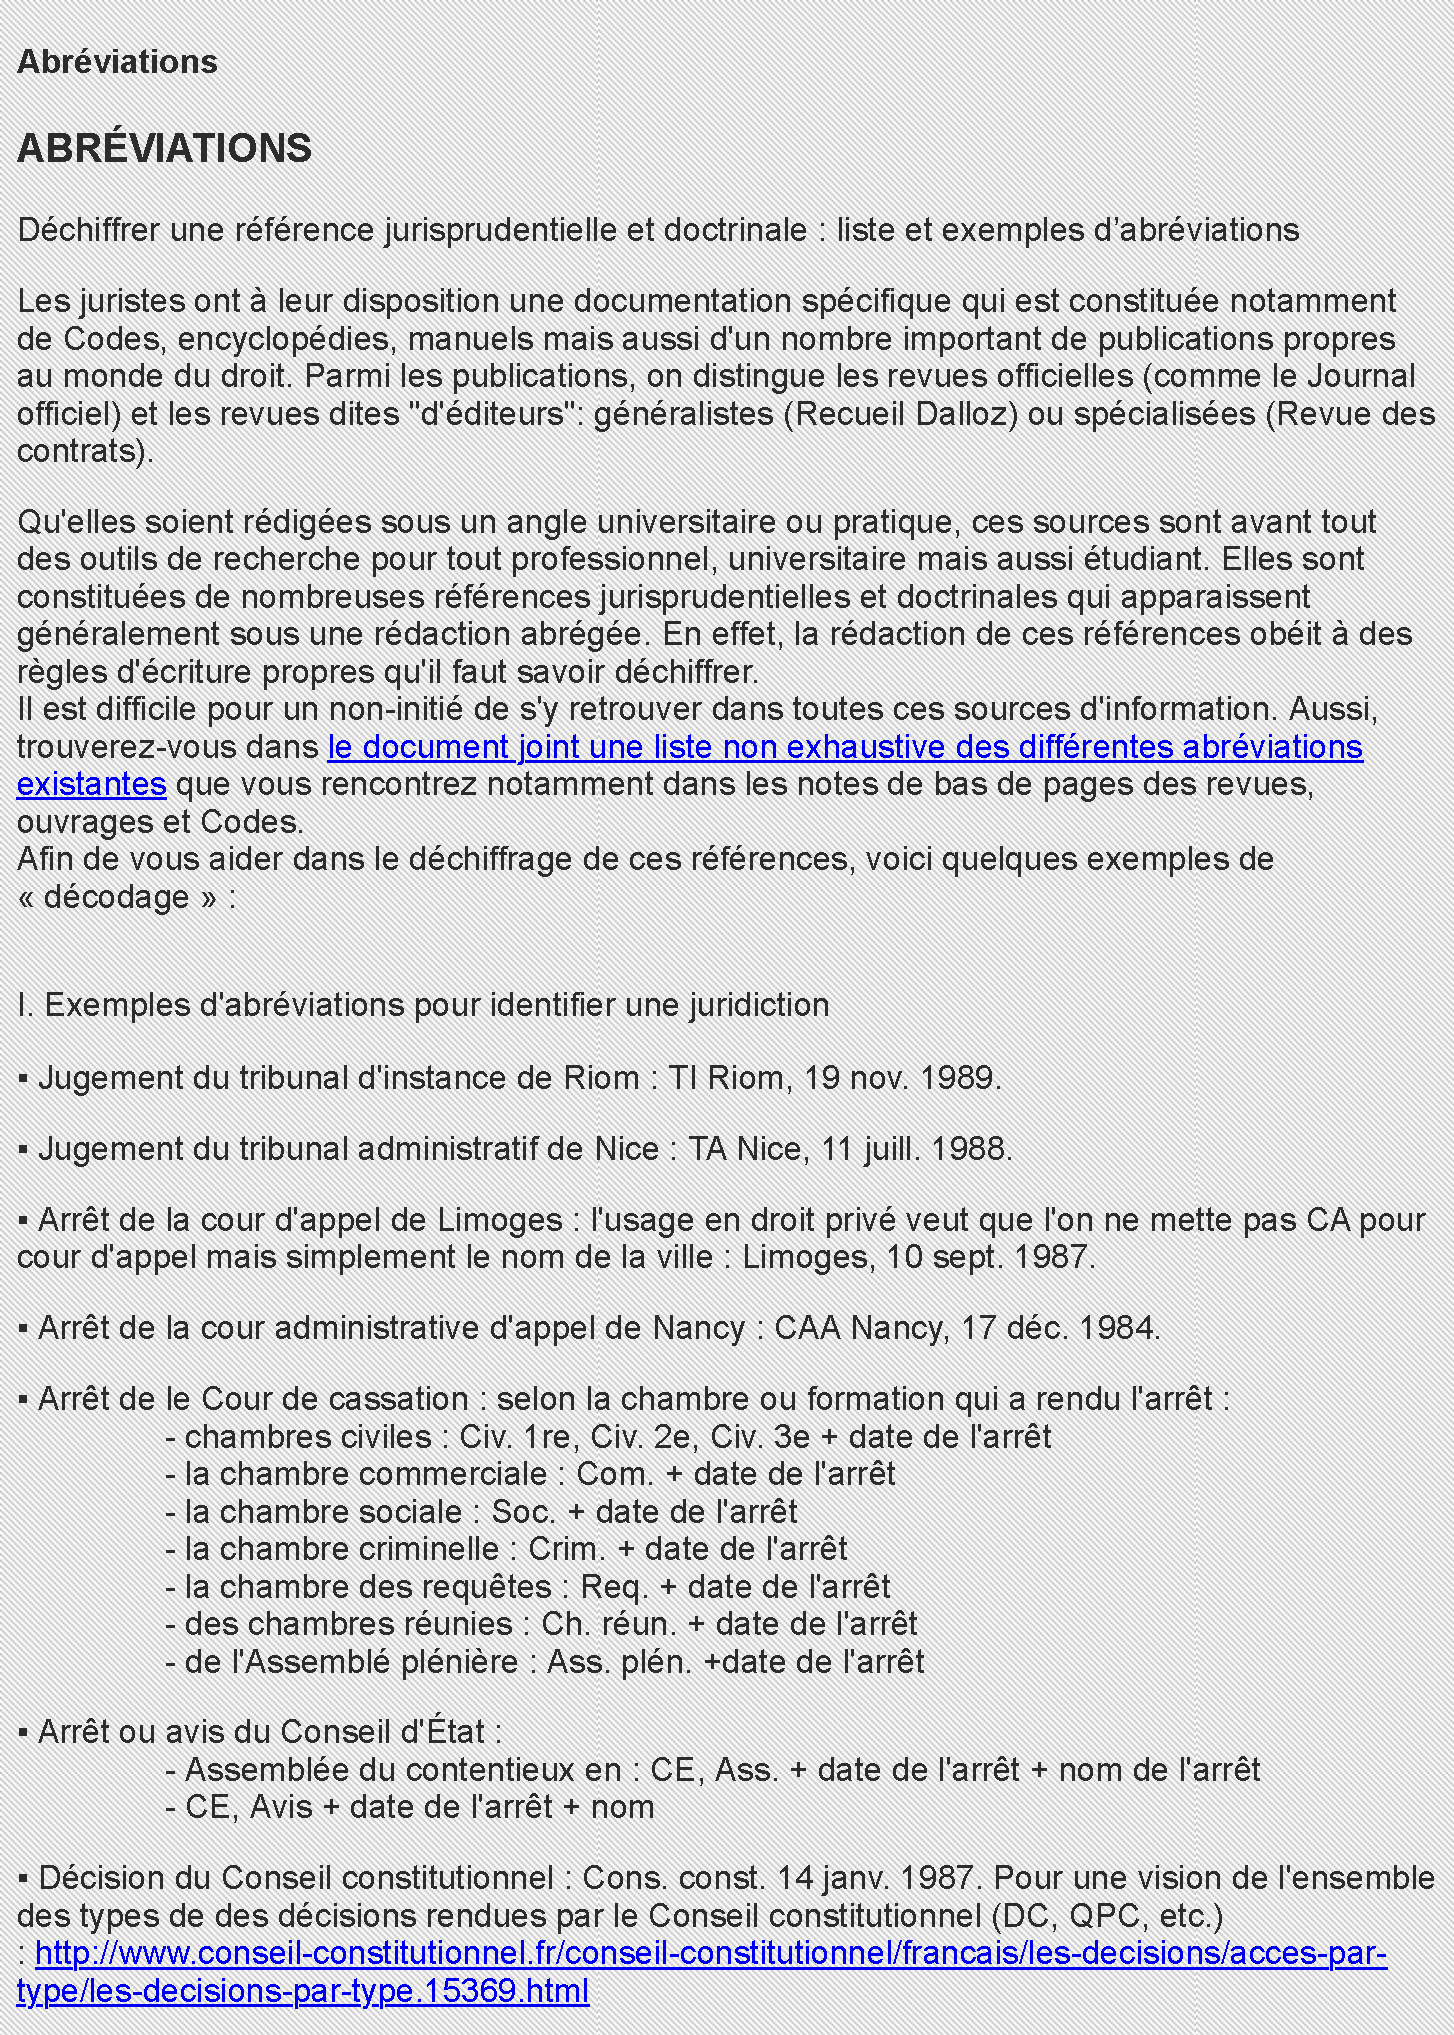
\includepdf[pages=-]{abreviations}

\end{document}
